\subsection{Artificial Neuron Introduction}

% figure of a bio neuron

The human brain is composed of billions of neurons: interconnected electrically excitable cells that form the basis of our intelligence.  Each neuron has synapses that receive electrical signals from multiple other neurons.  If the sum of these inputs is greater than a certain value, the neuron fires, generating a voltage at its axon.  The axon, or the output of the neuron cell, is itself connected to a synapse of another neuron.  The interconnections of these neurons form a massive network, where a huge number of inputs are processed in parallel to a set of outputs.  The basis of artificial neural networks is to simulate the mathematical properties of these neurons in order to perform similar tasks of mass parallel computation.

\begin{figure}[ht]
	\centering
	\def\layersep{2.5cm}
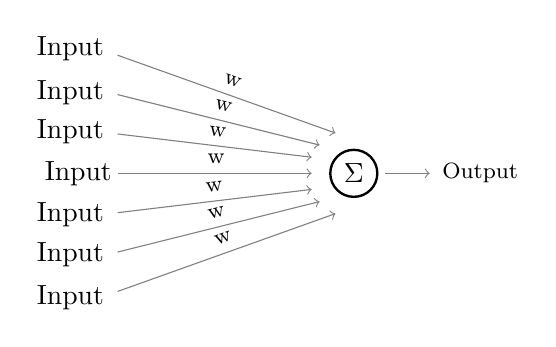
\begin{tikzpicture}[shorten >=1pt,->,draw=black!50, node distance=\layersep]
    \tikzstyle{every pin edge}=[<-,shorten <=1pt]
    \tikzstyle{neuron}=[circle,line width=0.3mm,draw=black,minimum size=17pt,inner sep=0pt]
    \tikzstyle{annot} = [text width=4em, text centered]


    \draw[->] (-3,1.5) -- (-.2,.5) node[sloped,midway,above] {\footnotesize w} node[left=3.4cm,above=.8cm]{Input};
    \draw[->] (-3,1) -- (-.4,.35) node[sloped,midway,above] {\footnotesize w} node[left=3.2cm,above=.4cm]{Input};
    \draw[->] (-3,0.5) -- (-.5,.2) node[sloped,midway,above] {\footnotesize w} node[left=3.1cm,above=.05cm]{Input};
    \draw[->] (-3,0) -- (-.5,0) node[sloped,midway,above] {\footnotesize w} node[left=2.45cm]{Input};
    \draw[->] (-3,-0.5) -- (-.5,-.2) node[sloped,midway,above] {\footnotesize w} node[left=3.1cm,below=.05cm]{Input};
    \draw[->] (-3,-1) -- (-.4,-.35) node[sloped,midway,above] {\footnotesize w} node[left=3.2cm,below=.4cm]{Input};
    \draw[->] (-3,-1.5) -- (-.2,-.5) node[sloped,midway,above] {\footnotesize w} node[left=3.4cm,below=.8cm]{Input};
    
    \node[neuron] (0,0) {$\Sigma$};

    \draw[->] (.4,0) -- (1,0) node[right] {\footnotesize Output};
\end{tikzpicture}
	\caption{Single Neuron Diagram}
\end{figure}

An artificial neuron simply a mathematical model of a biological neuron, and therefore its functionality is very similar.  Each neuron has multiple inputs, each with an individual weight, and one output.  The weight of an input is simply a positive or negative fraction that govern the impact of each input on the single output.  An artificial neuron's set of weights determines its function, and the function of each neuron in a neural network (in addition to the arrangement of the network) determines the function of the network as a whole.  This will become important as we discuss training Fido's neural network, however for the moment we will adjust our focus to the output of an artificial neural network.  By summing each input multiplied by its individual weight we reach a value called the activation, expressed as such mathematically for each input $x$ and weight $w$:

\begin{equation}
	a=\sum_{i=0}^{i=n}x_i w_i
	\,.
\end{equation}

If this activation value is less than a certain threshold, the output is zero.  If it is greater than the threshold, the output is one.  This activation function most closely resembles the biological model of a neuron, a binary step function.  However, a binary output can be somewhat limiting for many applications of neural networks.  For example, many of Fido's outputs are gradient rather than linear; as an example, an LED can be given a brightness.  For this purpose alternate activation functions can be used with gradient outputs.  One such function is a sigmoid function, expressed as such:

\begin{equation}
	O(a) = \cfrac{1}{1+e^{-\frac{a}{p}}}
	\,,
\end{equation}

\noindent for each output $O$, activation $a$, and constant $p$.  The sigmoid activation function can also be graphed as below.

\begin{figure}[ht]
	\centering
	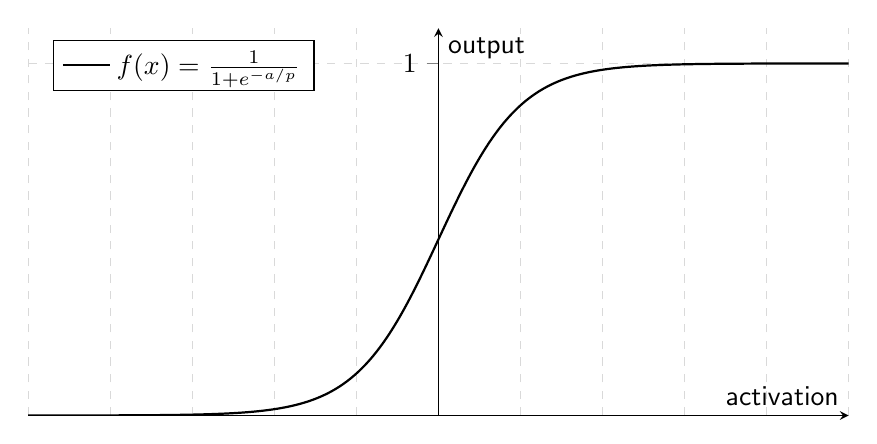
\begin{tikzpicture}[font=\sffamily]
    \begin{axis}[
    	legend pos=north west,
        axis x line=middle,
        axis y line=middle,
        grid = major,
        width=12cm,
        height=6.5cm,
        grid style={dashed, gray!30},
        xmin=-1,xmax= 1,ymin= 0,ymax= 1.1,
        xlabel=activation,ylabel=output,
        tick align=outside,
        ytick={1},
        xmajorticks=false,
        enlargelimits=false]
      \addplot[domain=-1:1,black,thick,samples=500] {1/(1+exp(-10*x))}; 
      \addlegendentry{$f(x)=\frac{1}{1+e^{-a/p}}$}
    \end{axis} 
\end{tikzpicture}
	\caption{Sigmoid Function Graph}
\end{figure}

This provides us with a gradient output, however output is still limited to positive values.  An alternative activation function which allows outputs ranging from -1 to +1 is the hyperbolic tangent activation function:

\begin{equation}
	O(a) = \tanh(a)% = \cfrac{e^a-e^{-a}}{e^a+e^{-a}}
	\,.
\end{equation}

The hyperbolic tangent activation can be graphed as such, demonstrating its greater range and gradient output.

\begin{figure}[ht]
	\centering
	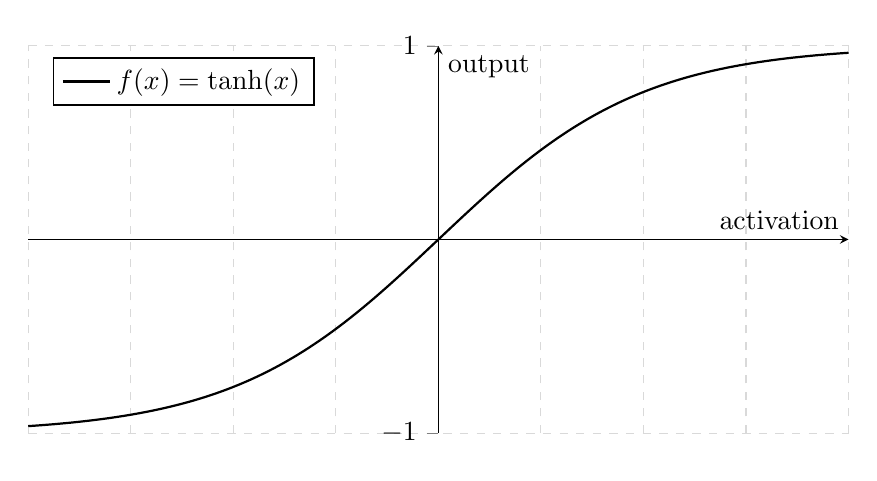
\begin{tikzpicture}
    \begin{axis}[
    	legend pos=north west,
        axis x line=middle,
        axis y line=middle,
        grid = major,
        width=12cm,
        height=6.5cm,
        grid style={dashed, gray!30},
        xmin=-2,xmax= 2,ymin= -1,ymax= 1,
        xlabel=activation,ylabel=output,
        tick align=outside,
        ytick={-1,1},
        xmajorticks=false,
        enlargelimits=false]
      \addplot[domain=-2:2,black,thick,samples=500] {tanh(x)}; 
      \addlegendentry{$f(x)=\tanh(x)$}
    \end{axis} 
\end{tikzpicture}
	\caption{Hyperbolic Tangent Function Graph}
\end{figure}

\subsection{Feedforward Neural Network}

A traditional method of arranging artificial neurons in a neural network is called a feedforward network.  Neurons are connected as previously described: the output of each neuron is connected to one of the inputs of another neuron.  These neurons are organized into layers, as described in the following figure: % ogres have layers

\begin{figure}[ht]
	\centering
	\def\layersep{2.5cm}
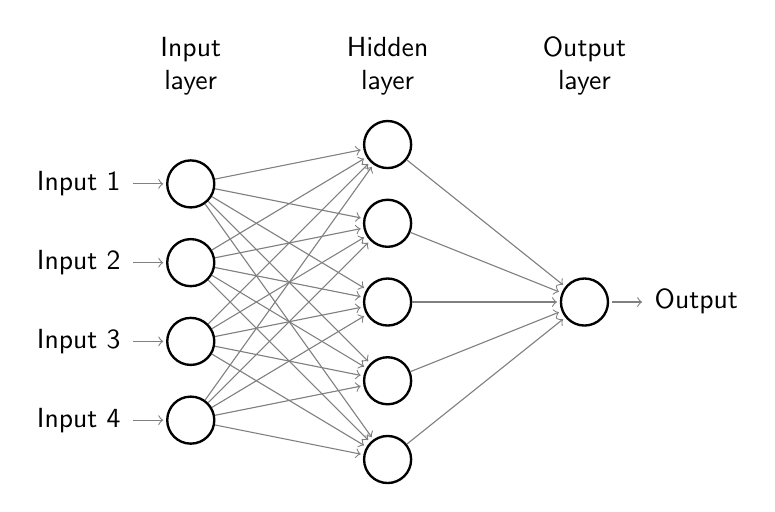
\begin{tikzpicture}[shorten >=1pt,->,draw=black!50, node distance=\layersep,font=\sffamily]
    \tikzstyle{every pin edge}=[<-,shorten <=1pt]
    \tikzstyle{neuron}=[circle,line width=0.3mm,draw=black,minimum size=17pt,inner sep=0pt]
    \tikzstyle{annot} = [text width=4em, text centered]

    \foreach \name / \y in {1,...,4}
        \node[neuron, pin=left:Input \y] (I-\name) at (0,-\y) {};

    \foreach \name / \y in {1,...,5}
        \path[yshift=0.5cm]
            node[neuron] (H-\name) at (\layersep,-\y cm) {};

    \node[neuron,pin={[pin edge={->}]right:Output}, right of=H-3] (O) {};

    \foreach \source in {1,...,4}
        \foreach \dest in {1,...,5}
            \path (I-\source) edge (H-\dest);

    \foreach \source in {1,...,5}
        \path (H-\source) edge (O);

    %\draw[->] (5,-2.9) -- (5,-5) -- (1,-5) -- (1,-4.5);
    %\node (1,-4.5) {Error back propagation}

    \node[annot,above of=H-1, node distance=1cm] (hl) {Hidden layer};
    \node[annot,left of=hl] {Input layer};
    \node[annot,right of=hl] {Output layer};
\end{tikzpicture}
	\caption{Single Output Feedforward Network}
\end{figure}

Initial inputs are first sent into the input layer.  Next, the output of each input layer neuron is sent into each neuron in the hidden layer.  The hidden layer processes the inputs to outputs using an activation function and a weight value for each input.  There can be any number of hidden layers in a neural network, depending on the complexity of the computation being performed.  Finally the outputs from the last hidden layer neurons are sent into each neuron of the output layer, where the final outputs are processed.  A concrete example of a feedforward network is that of Fido.  Sensor inputs such as light and sound are sent into the input layer.  After the signals have passed through to the output layer, the outputs from the output layer are sent to outputs such as motors, LEDs, and buzzers.   The purpose of training a neural network is to make input values correspond to the correct output values, depending on the desired behavior.  An example could be making Fido drive when light is applied.  The way to give a neural network desired behavior is by controlling the weights of each neuron using a learning algorithm.